\documentclass[10pt]{article}
\usepackage{eecs149}
\usepackage{multicol,caption,hyperref}
\usepackage[margin={2cm,2cm}]{geometry}
\newenvironment{Figure}
  {\par\medskip\noindent\minipage{\linewidth}}
  {\endminipage\par\medskip}
\tikzset{
  >=stealth'
}
\def\videolink{\url{https://www.youtube.com/watch?v=slTO1ecGoM0}}
\begin{document}
\begin{center}
  \Large Gesture Controlled Driving
\end{center}
\begin{center}
  Ollie Peng, Manish Raghavan, Victor Sutardja \\
  Video Demonstration: \videolink{}
\end{center}
\begin{multicols*}{2}
  \section*{Overview}
  Using the Kobuki platform from lab, we built a system by which the Kobuki
  drives in a path drawn by the user. Specifically, the user draws a path in the
  air using a brightly colored object. The Kobuki takes a series of images of
  this path using a webcam mounted on its frame. These images are streamed to a
  laptop which performs the image-processing needed to detect the object used
  for drawing. The points from the images are interpolated into a smooth path.
  Using feedback from the OptiTrack camera system, the Kobuki is instructed to
  drive along this path, correcting for any errors in real time.

  \section*{Setup}
  \begin{Figure}
    \begin{tikzpicture}[->,shorten >=1pt,auto,node distance=2cm, thin]
      \node (m) [rectangle,draw] at (0,0) {Mac};
      \node (k) [rectangle,draw] at (2,0) {Kobuki};
      \node (w) [rectangle,draw] at (-3.5,0) {Windows};
      \node (o) [rectangle,draw] at (-3.5,2) {OptiTrack};

      \path
      (k) edge [bend right=30] node [above,align=center] {images;\\orientation}
      (m)
      (m) edge [bend right=30] node [below] {radius and speed} (k)
      (w) edge node [below,align=center] {position and\\orientation} (m)
      (o) edge node [right,align=center] {full tracking\\data} (w)
      ;
    \end{tikzpicture}
    \captionof{figure}{Flow of information} \label{fig:info}
  \end{Figure}

  Figure~\ref{fig:info} shows the flow of information between various devices.
  There are two key design decisions we made in order to overcome challenges we
  faced. First, we streamed the OptiTrack data to a separate Windows machine
  instead of the Mac that was communicating with the data because the frame rate
  from the traking system was too high and would be constantly modifying shared
  variables. Since we were only sending updated commands to the Kobuki once
  every second, we did not need such frequent information, and therefore used
  the Windows machine to sample the data at a lower rate before passing it on
  the Mac. Second, we chose to take orientation data from both the OptiTrack and
  Kobuki. We did so because the orientation from OptiTrack was given in terms of
  quaternions in a rotated axis space, meaning that the standard equations for
  converting to yaw, pitch, and roll no longer applied. Instead, we needed to
  know which quadrant the yaw was in to correct them. As a result, we used the
  orientation from the Kobuki to determine which quadrant it was facing,
  allowing us to use the correct equations to get the true orientation.

  \section*{Image Processing}
  The first step to converting the drawn gesture to some sort of path is to
  capture key points along the gesture's trajectory. We set up a simple LabVIEW
  system to take a series of RGB pictures using the color camera attached to the
  myRIO. For each picture, we then apply a color threshold to mask out areas of
  the image with the wrong color. This leaves us with one or more contours of
  the correct color in our image. We can then construct a list of these contours
  and then iterate over the list to find the largest such contour, which will
  almost always correspond to the object we are trying to track. Since we want
  each image to identify just a single point on the path, we turn to the
  centroid $(\overline{x}, \overline{y})$, the arithmetic mean position of all
  points within the contour $P$, which we calculate using moments of the
  contour: \cite{centroid}

  $$(\overline{x}, \overline{y}) = \p{\frac{m_{10}}{m_{11}},
  \frac{m_{01}}{m_{00}}}$$
  where
  $$m_{ij} = \sum_{\mathbf{p} \in P} \mathbf{p} \cdot x^i \cdot y^j$$

  With all the images processed, this gives us an ordered list of $(x, y)$
  coordinates that quite accurately represent the complete gesture.

  In Figure~\ref{fig:thresh}, the color thresholding identifies two main point
  clouds: the actual object and the controller's face. However, by identifying
  the contours of these clouds, we detect the larger of the two clouds and find
  the centroid of that, making our detection resilient to noisy images.
  \begin{Figure}
    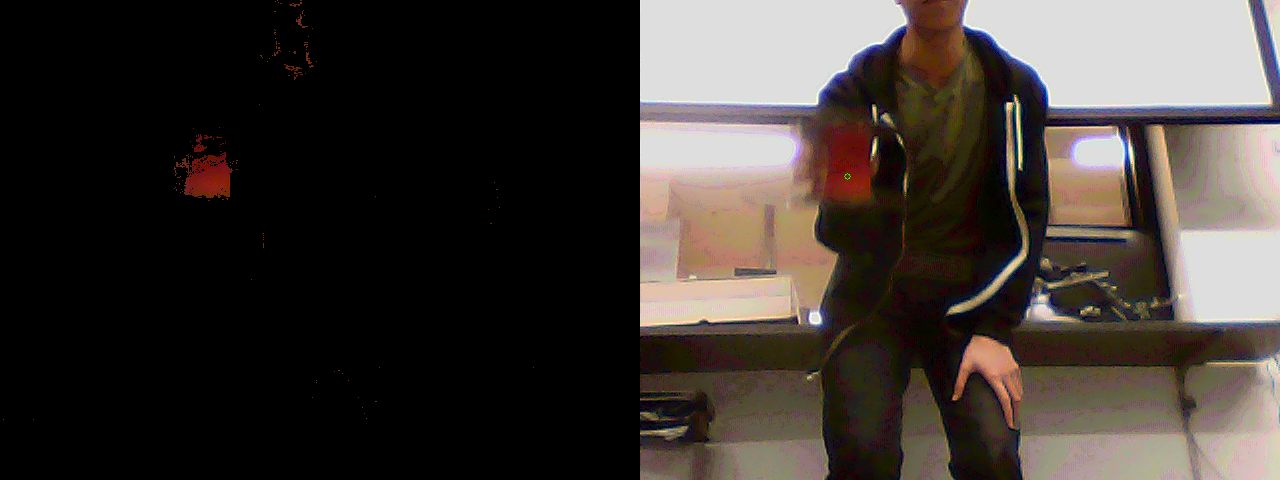
\includegraphics[width=9cm]{../thresh_img/detect5.png}
    \captionof{figure}{Detecting an object} \label{fig:thresh}
  \end{Figure}

  \section*{B-spline Interpolation}
  We chose B-spline interpolation with cubic polynomials because it has the
  following properties: \cite{fuhuacheng2012}
  \begin{itemize}
    \item Locality -- only nearest 4 points affect the curve
    \item Continuity -- continuous up to the second derivative despite being
      piecewise defined
  \end{itemize}
  B-spline interpolation yields a smooth path, allowing the Kobuki to drive
  without stopping to turn. Intuitively, the interpolation yields a path that is
  at any time a linear combination of three neighboring points, weighted by the
  basis curves at those points. Since the basis curves, shown in
  Figure~\ref{fig:basis} approximate Gaussians in the middle of the path (i.e.
  the curve shown in light blue), the interpolation can be viewed as letting
  each control point have ``influence'' on the interpolated curve that depends
  on how close the curve is to that point. However, this means that the
  interpolated curve does not actually pass through the control points. As a
  result, we had to take in a series of data points and find control points such
  that the resultant curve interpolated through the control points passes
  through the original data points. Figure~\ref{fig:sample} shows how from the
  original data points, shown in blue, a series of control points, shown in red,
  are computed, and when interpolated, the final path passes through the data
  points.

  By convention, we will assume that we have $n+1$ data points $\mathbf{D}_0,
  \dots, \mathbf{D}_n$. To ensure that the endpoints of the curve are correct,
  we define \[t_i = \begin{cases}
      0 & 0 \le i \le 3 \\
      i-3 & 3 \le i \le n+3 \\
      n+3 & n+3 \le i \le n+6
    \end{cases}
  \]
  The equations for the basis functions are given by the following recurrence
  relation: \cite{wiki:spline}
  \[N_{i,1}(x) \coloneqq \begin{cases}
      1 &\text{ if } t_i \le x < t_{i+1} \\
      0 &\text{ otherwise}
  \end{cases} \]
  \begin{align*}
    N_{i,k}(x) &\coloneqq \frac{x-t_i}{t_{i+k-1}-t_i} N_{i,k-1}(x) \\
    &+ \frac{t_{i+k}-x}{t_{i+k}-t_{i+1}} N_{i+1,k-1}(x)
  \end{align*}
  In order to get the curve to pass through all the data points, we need 2 more
  control points than data points. To find the control points $\mathbf{P}_0,
  \dots, \mathbf{P}_{n+2}$ from the data points, we use the fact that the curve
  must start and end with our first and last data points and must pass through
  each of our data points. Since we have $n+3$ control points and $n+1$ data
  points, we add the initial conditions that the second derivative of the curve
  at the start and end points must be 0. This yields the following system of
  equations:
  \begin{align*}
    \mathbf{P}_0 &= \mathbf{D}_0 \\
    \frac{3}{2} \mathbf{P}_1 - \frac{1}{2} \mathbf{P}_2 &= \mathbf{D}_0 \\
    N_{i,4}(i) \mathbf{P}_i + N_{i+1,4}(i) \mathbf{P}_{i+1} + N_{i+2,4}(i)
    \mathbf{P}_{i+2} &= \mathbf{D}_i \\
    -\frac{1}{2} \mathbf{P}_{n} - \frac{3}{2} \mathbf{P}_{n+1} &= \mathbf{D}_n \\
    \mathbf{P}_{n+2} &= \mathbf{D}_{n}
  \end{align*}
  To interpolate the curve from the control points, we simply use
  \[C(t) = \sum_{i=0}^{n+2} N_{i,4}(t) \mathbf{P}_i\]
  Note that for any value of $t$, at most 4 of the $N_{i,4}$ values are nonzero
  (see Figure~\ref{fig:basis}), meaning the curve only depends on the nearest 4
  control points.

  \begin{Figure}
    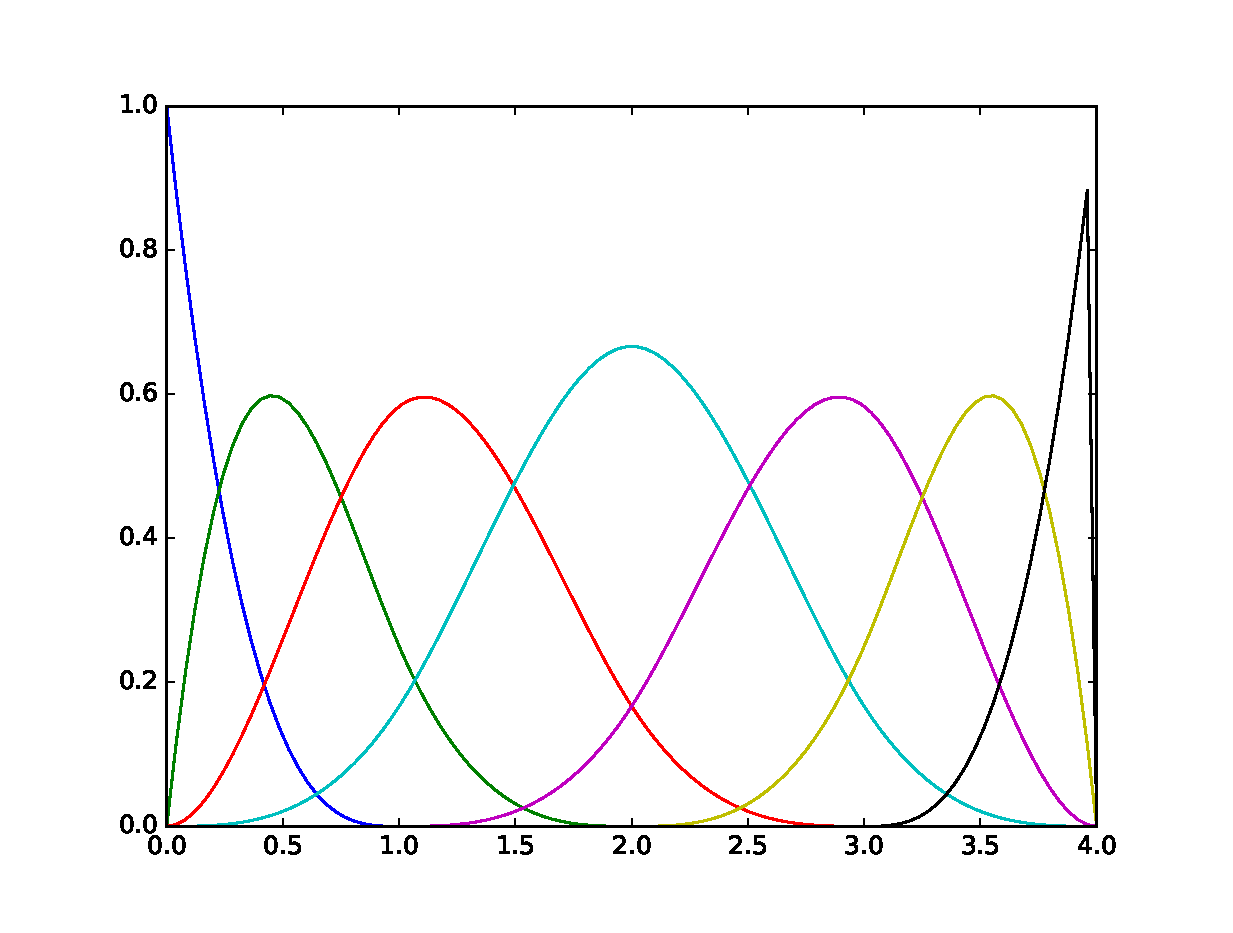
\includegraphics[width=9cm]{../spline_basis.eps}
    \captionof{figure}{Cubic spline basis curves} \label{fig:basis}
  \end{Figure}
  \begin{Figure}
    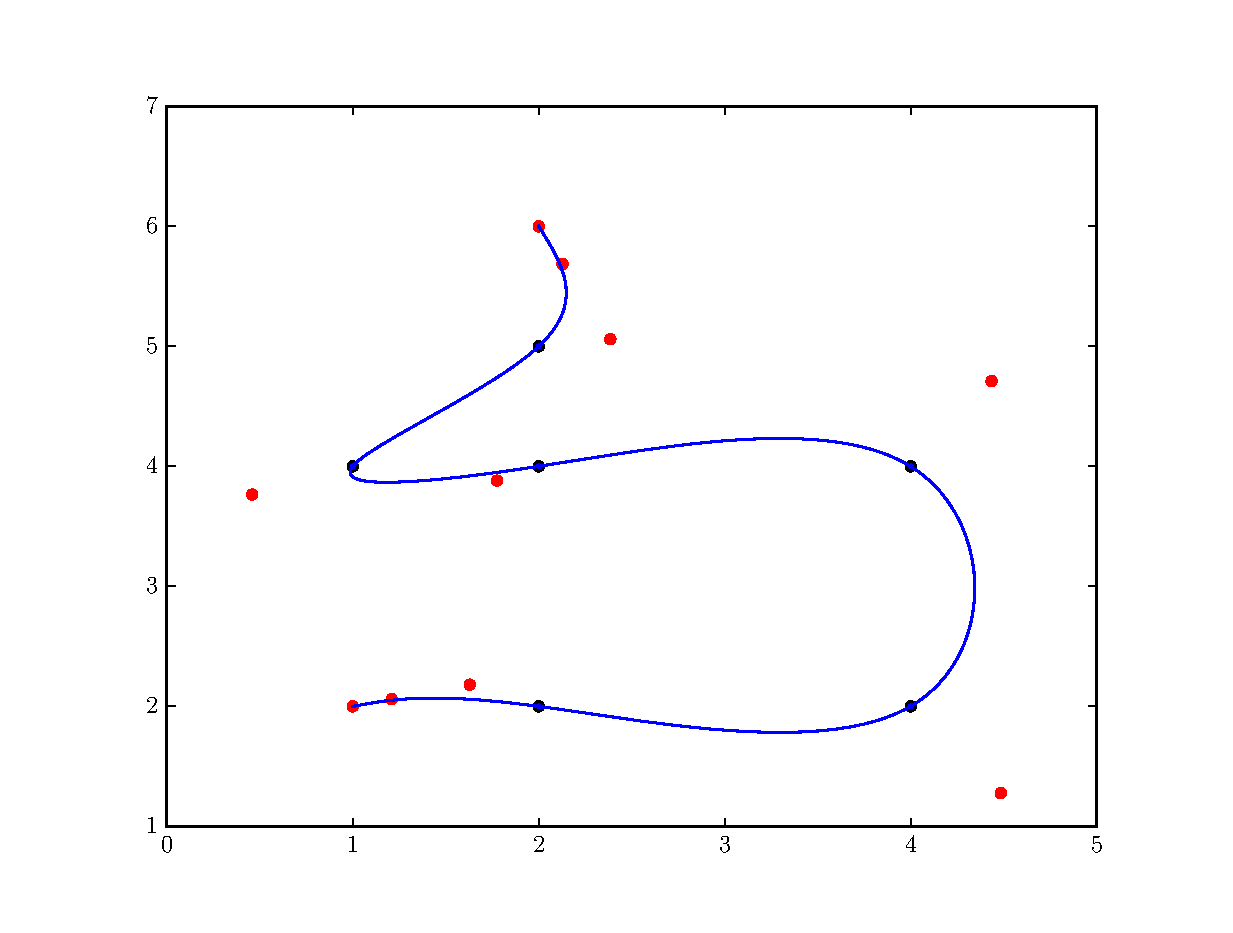
\includegraphics[width=9cm]{../s_img/spline8.eps}
    \captionof{figure}{Sample cubic spline interpolation} \label{fig:sample}
  \end{Figure}

  \section*{Timing}
  All the communication between the various systems we used had to be timed in
  such a way that the latency between the arrival of new data and its usage was
  low. The main limiting factor was that on the Kobuki, polling a socket for new
  data too frequently could sometimes prevent any changes in wheel speed from
  taking effect. In order to fix this, we made the Kobuki poll for new data
  every 960 ms. Data was sent by the Mac once a second, meaning the average
  latency between commands being issued and received was around half a second.
  Since the Mac was multithreaded, it polled orientation data from the Kobuki
  every 200 ms, meaning latency in this case was based on how frequently the
  Kobuki sent data (every 960 ms). Since these two were connected directly by a
  shared WiFi network from the Mac, the network latency was negligible compared
  to this. The OptiTrack frame rate was actually too high, so the Windows
  machine sampled every 10 frames and sent those to the Mac over a direct
  ethernet connection, which were then further sampled once a second. Since the
  frames were generated so frequently, a frame read by the Mac was in the worst
  case on the order of tens of milliseconds old. Overall, the latency between
  data being generated by OptiTrack and the Kobuki's wheen speeds being udpated
  was in the worst case no more than around 1.2 seconds, which was sufficient to
  produce a path with low error.

  \section*{Threading}
  In controlling the Kobuki, we had to send it instructions while also receiving
  orientation data from it. To do so, we used threading -- one thread listened
  for data from the Kobuki while the other thread used that data to control it.
  In order to prevent race conditions, we used locks on two shared resources:
  the socket over which we were communicating and a global variable containing
  the Kobuki's orientation. Since we had two threads each using the same two
  locks, we had to avoid deadlock, which we did by ensuring that no thread held
  more than one lock at the same time. Each thread executed a task periodically,
  on the order of tenths of a second or longer, meaning that the delay caused by
  waiting for locks was insignificant compared to the running time allowed for
  each task.

  \section*{Modeling Movement and Control}
  The Kobuki requires a radius of curvature and wheel speed to control its
  motion. Our control algorithm takes in the Kobuki's current position, the next
  position it should go to, its current orientation to produce these quantities.
  Let $\mathbf{p}_1 = (x_1, y_1)$ be the Kobuki's current position and
  $\mathbf{p}_2 = (x_2, y_2)$ be the Kobuki's next position. Let
  $\mathbf{p}_{\Delta} = \mathbf{p}_2 - \mathbf{p}_1$. Let $\phi$ be its
  current orientation, measured counterclockwise from the positive $x$ axis. The
  angle $\alpha$ between its current position and its next position is given by
  \begin{align*}
    \alpha &= \text{sign}(y_{\Delta})
    \arccos\p{\frac{x_{\Delta}}{||\mathbf{p}_{\Delta}||}}
  \end{align*}
  The total angle it must turn is $\theta = \alpha - \phi$. The radius of
  curvature is then given by $r = \frac{||\mathbf{p}_{\Delta}||}{2\sin \theta}$,
  which is positive if turning left and negative otherwise. The angle through
  which it must follow an arc of this circle to reach $\mathbf{p}_2$ is $2
  \theta$, so the speed at which it must travel is $s = \frac{2r\theta}{\tau}$,
  where $\tau$ is the time alotted for it to reach $\mathbf{p}_2$.
  Figure~\ref{fig:roc} shows the model of the Kobuki's path from $\mathbf{p}_1$
  to $\mathbf{p}_2$.

  \begin{Figure}
    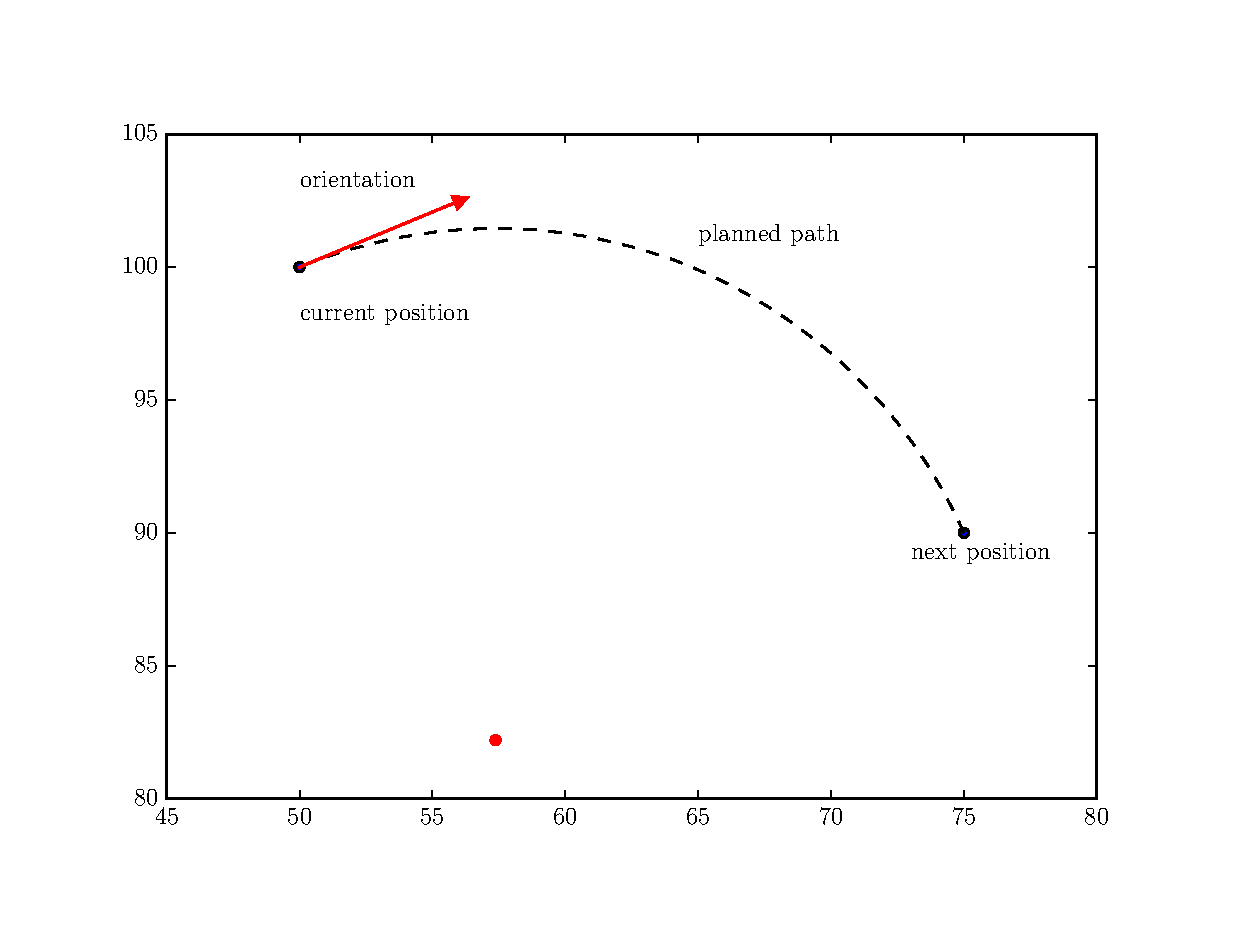
\includegraphics[width=9cm]{../plots/roc.eps}
    \captionof{figure}{Movement planning} \label{fig:roc}
  \end{Figure}

  As long as $\theta$ is small, the path produced is small and does not
  oscillate. However, for paths along which the radius of curvature changes
  drastically (meaning the third derivative of the interpolated path is high),
  $\theta$ can become larger, causing the Kobuki to get off course.

  \section*{Challenges}
  One of the major issues we faced was communication between devices over
  networks we could not control. Because AirBears2 blocks traffic on some ports,
  we had to set up our own local networks, while remaining connected to the
  Internet to stream OptiTrack data. In such a complex network, new problems
  arose arbitrarily as factors outside our control made our communications
  unpredictable.

  Another challenge we faced was getting the Kobuki's orientation from
  OptiTrack. The OptiTrack system sends the orientation in terms of quaternions,
  with two major issues: the axis that OptiTrack uses is nonstandard (the $y$
  axis points up instead of $z$) and every so often the system randomly
  perceives that the Kobuki has flipped over $180^{\circ}$, meaning the
  orientation suddenly becomes negative. To solve these challenges, we did the
  following:
  \begin{enumerate}
    \item Calculated the yaw using the standard equation for pitch:
      \cite{wiki:quat}
      $$\theta = \arcsin\p{2(q_w q_y - q_x q_z)}$$
    \item Since $\arcsin$ returns a result between $-\frac{\pi}{2}$ and
      $\frac{\pi}{2}$, we took orientation data from the Kobuki as well to
      determine if it was facing in the positive or negative $x$ direction,
      calculating the overall yaw to be $\theta$ or $\pi-\theta$ in the two
      cases respectively.
  \end{enumerate}
  This allowed us to continue to use the more accurate OptiTrack data, only
  using the Kobuki's orientation to corroborate the data sent by OptiTrack.

  \section*{Results}
  Figures~\ref{fig:circ_plot} and~\ref{fig:s_plot} depict examples of the
  Kobuki's actual path (shown in blue) compared to the planned path (shown in
  red), as tracked by the OptiTrack system.

  For the path shown in Figure~\ref{fig:circ_plot}, the RMS deviation from the
  path is 6.074 mm. The deviation occurs because the Kobuki is always in a sense
  ``catching up'' to where it should be on the path, so it tends to cut the
  corners. In Figure~\ref{fig:s_plot}, the RMS deviation rises to 14.293 mm
  because the radius of curvature must change much more quickly.

  \begin{Figure}
    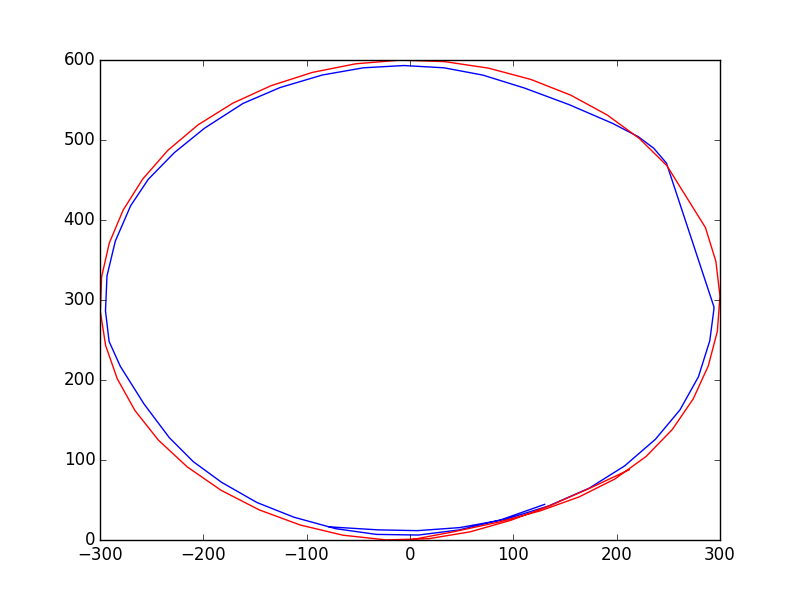
\includegraphics[width=9cm]{../plots/circle_plot.png}
    \captionof{figure}{Actual vs. planned path with low third derivative}
    \label{fig:circ_plot}
  \end{Figure}

  \begin{Figure}
    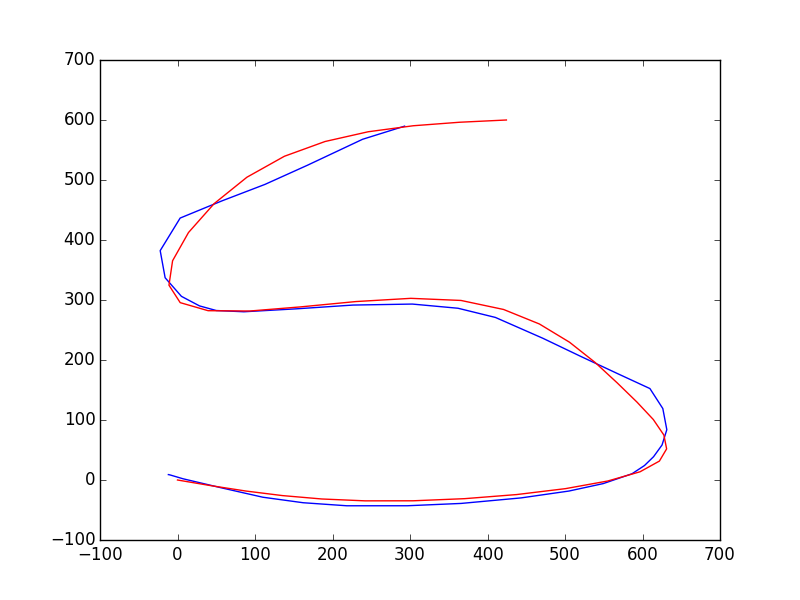
\includegraphics[width=9cm]{../plots/s_plot.png}
    \captionof{figure}{Actual vs. planned path with high third derivative} \label{fig:s_plot}
  \end{Figure}

  A video of the Kobuki following the path shown in Figure~\ref{fig:s_plot} can
  be found at \videolink{}

  \section*{Extensions}
  In order to improve performance on instances with high third derivatives, we
  could either send commands to the Kobuki more frequently or reduce the speed
  at which the Kobuki to follows the path. Doing either would allow us to react
  to deviations from the true path more quickly, thus reducing the overall
  error. We could also modify the control algorithm to create a plan that looks
  beyond just the next point -- for example, we could consider the desired
  orientation upon reaching the next point. This would allow the planned route
  to better approximate the actual path, reducing error.

  Since our final control algorithm only used position, next position, and
  orientation, it could be easily extended to allow the Kobuki to follow a
  moving object. As long as the Kobuki's position and orientation are sampled
  frequently enough, it could follow a moving object using the same techniques.
\end{multicols*}
\bibliographystyle{plain}
\bibliography{refs}
\end{document}
